\exercise{Coordinate shift\label{exGeneratingCoordshift}}{2}
Consider the function $f(x)=\sqrt{x}$. We are going to approximate the function around the point $x^*=1$.

\subquestion
Introduce a new variable $y$, such that the point of interest ($x^*=1$) is at $y^*=0$. 

\solution 
We define 
\eq{y=x-1.}
Using this relation we can confirm that $x^*=1$ corresponds to $y^*=0$.

\subquestion
Write $f$ in terms of $y$, call the resulting function $h(y)$.

\solution 
We can solve the defining equation of $y$ for $x$, which yields
\eq{
x=y+1.
}
Substituting this equation into $f$ yields 
\eq{
f(x)=\sqrt{x}=\sqrt{y+1}=h(y)
}
\subquestion
Approximate $h(y)$ by a function of the form $g(y)=c_0+c_1y$ around $y^*=0$.

\solution
To find $c_0$ we evaluate $h$ at $y^*=0$. Let's write this using the bar notation 
\eq{
c_0 = h(0) = \left. \sqrt{y+1} \right|_{y=0} = \sqrt{1}=1. 
}
To find $c_1$ we differentiate and thereafter substitute the $y=0$
\eq{
c_1 = h'(0) = \left. \frac{\partial}{\partial y } \sqrt{y+1} \right|_{y=0} = \frac{1}{2\sqrt{1}} = \frac{1}{2} 
}
hence
\eq{
h(y)\approx g(y)=1+\frac{1}{2}y.
}

\subquestion
Write the approximation in terms of the original variable $x$.

\solution
We translate back to $x$ by using the definition of $y$ in the form $y=x-1$. Substituting into $g(y)$ yields 
\eq{
f(x)\approx 1+\frac{1}{2} (x-1) 
}
which we can simplify to 
\eq{
f(x)\approx \frac{1}{2}+\frac{1}{2}x 
}
Here is a plot of the approximation for you:
\begin{center}
    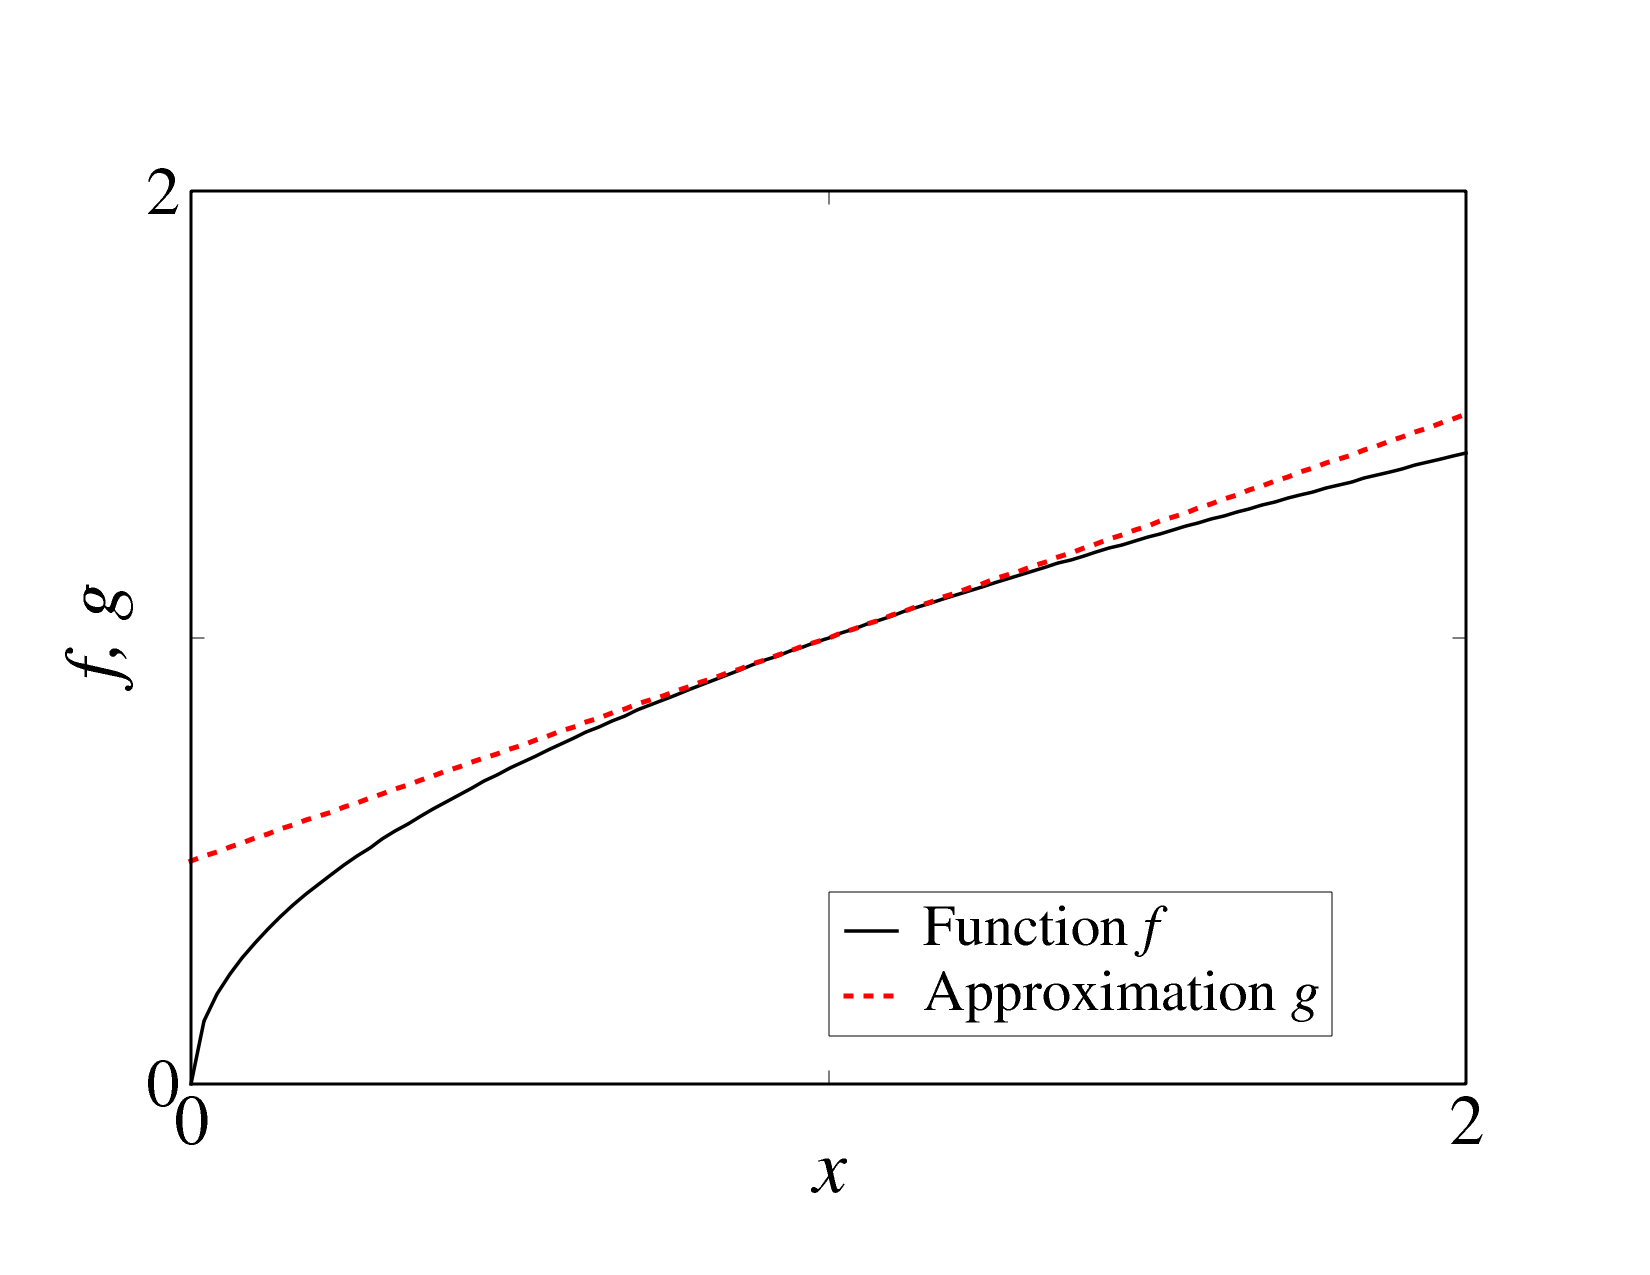
\includegraphics[width=0.6\textwidth]{approximation1}
\end{center}

\subquestion Apply the same steps to approximate $f$ up to quadratic order around $x^*=2$.

\solution
In this case we need to define 
\eq{
y=x-2,
}
Substituting $x=y+2$ into $f$ gives us 
\eq{
f(x)=\sqrt{x}=\sqrt{y+2}=h(y).  
}
We are looking for an approximation of the form 
\eq{
g(y)=c_0+c_1y+c_2y^2
}
We find $c_0$ in the usual way
\eq{
c_0=h(0)=\sqrt{2}.
}
Furthermore we know,
\eq{
c_1=h'(0)=\frac{1}{2\sqrt{2}}
}
For the quadratic term we have to be careful because an extra factor of 2 appears in the Taylor formula
\eqa{
c_2 &=& \frac{1}{2!}\left.\frac{\partial}{\partial y}h(y)\right|_{y=0} \\
   &=& \frac{1}{2}h''(0) \\
   &=& \frac{1}{2} \left.\frac{\partial}{\partial y} \frac{1}{2\sqrt{y+2}}\right|_{y=0} \\
   &=& \frac{1}{2} \left(-\frac{1}{4} (y+2)^{-\frac{3}{2}}\right)_{y=0} \\
   &=& -\frac{1}{8\sqrt{8}}    
}
So our solution in terms of $y$ is 
\eq{
h(y)\approx \sqrt{2} + \frac{y}{2\sqrt{2}} - \frac{y^2}{16\sqrt{2}}.
}
To find the solution in terms of $x$ we substitute $y=x-2$ which yields 
\eqa{
f(x)&\approx&\sqrt{2} + \frac{x-2}{2\sqrt{2}} - \frac{(x-2)^2}{16\sqrt{2}} \\ 
  &=& \frac{1}{\sqrt{2}}\left( 2 + \frac{x-2}{2} - \frac{(x-2)^2}{16}    \right) \\
  &=& \frac{1}{\sqrt{2}}\left( 2 + \frac{x}{2} -1 - \frac{x^2}{16}+\frac{x}{4}-\frac{(1}{4} \right) \\
  &=& \frac{1}{\sqrt{2}}\left( \frac{3}{4} + \frac{3}{4}x  - \frac{x^2}{16} \right) 
}
This doesn't look like multiplying it out will make it simpler, so we leave it at that. Here is a plot for this result:
\begin{center}
    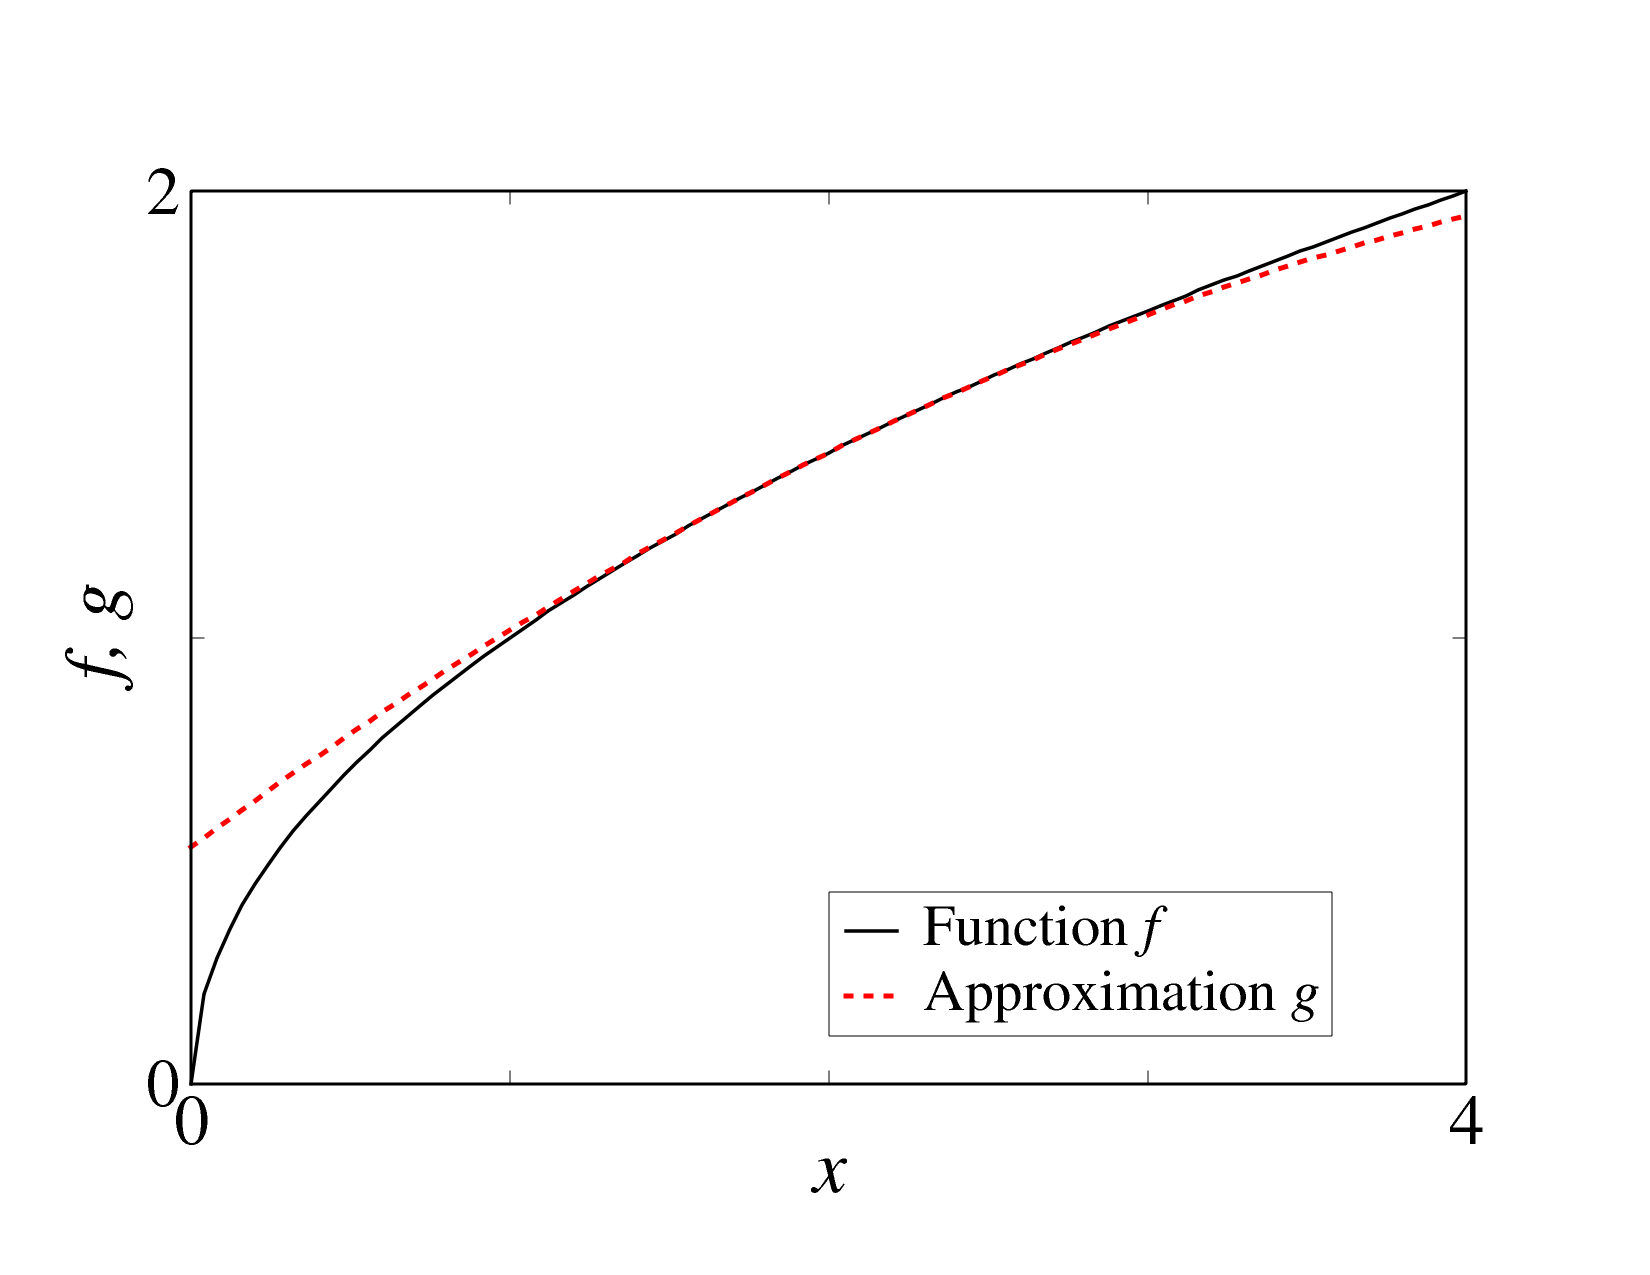
\includegraphics[width=0.6\textwidth]{approximation2}
\end{center}
